\chapter{Backpropagation}

\section{Feedforward Backpropagation Network}
The feedforward backpropagation network is a \textbf{very popular model} in neural
networks. It \textbf{does not have feedback connections}, but errors are
backpropagated during training. \textbf{Least mean squared error} is used. Many
applications can be formulated for using a feedforward backpropagation
network, and the methodology has been a model for most multilayer neural
networks. Errors in the output determine measures of hidden layer output
errors, which are used as a basis for adjustment of connection weights between
the input and hidden layers. Adjusting the two sets of weights between the
pairs of layers and recalculating the outputs is an iterative process that is
carried on until the errors fall below a tolerance level. Learning rate
parameters scale the adjustments to weights. A momentum parameter can also
be used in scaling the adjustments from a previous iteration and adding to the
adjustments in the current iteration.

\subsection{Mapping}
The feedforward backpropagation network maps the input vectors to output
vectors. Pairs of input and output vectors are chosen to train the network first.
Once training is completed, the weights are set and the network can be used to
find outputs for new inputs. The \textbf{dimension of the input vector determines} the
\textbf{number of neurons in the input layer}, and the \textbf{number of neurons in the output
layer} is determined by the \textbf{dimension of the outputs}. If there are $k$ neurons in
the input layer and $m$ neurons in the output layer, then this network can make a
mapping from $k$-dimensional space to an $m$-dimensional space. Of course,
what that mapping is depends on what pair of patterns or vectors are used as 
exemplars to train the network, which determine the network weights. Once
trained, the network gives you the image of a new input vector under this
mapping. Knowing what mapping you want the feedforward backpropagation
network to be trained for implies the dimensions of the input space and the
output space, so that you can determine the numbers of neurons to have in the
input and output layers.

\subsection{Layers}

The architecture of a feedforward backpropagation network is shown in Figure \ref{fig:simple_backpropagation}. While there can be many hidden layers, we will illustrate this network with only one hidden layer. Also, the number of neurons in the input layer and
that in the output layer are determined by the dimensions of the input and
output patterns, respectively. It is not easy to determine how many neurons are
needed for the hidden layer. In order to avoid cluttering the figure, we will
show the layout in Figure \ref{fig:simple_backpropagation} with four input neurons, three neurons in the
hidden layer, and one output neuron(s), with a few representative connections.
The network has three fields of neurons: one for input neurons, one for hidden
processing elements, and one for the output neurons. As already stated,
connections are for feed forward activity. There are connections from every
neuron in field A to every one in field B, and, in turn, from every neuron in
field B to every neuron in field C. Thus, there are two sets of weights, those
figuring in the activations of hidden layer neurons, and those that help
determine the output neuron activations. In training, all of these weights are
adjusted by considering what can be called a cost function in terms of the error
in the computed output pattern and the desired output pattern. \\
\def\layersep{2.5cm}
\begin{figure}[ht!]
\caption{An simple Backpropagation Network} 
\label{fig:simple_backpropagation}
\centering
\begin{tikzpicture}[shorten >=1pt,->,draw=black!50, node distance=\layersep]
    % Draw the input layer nodes
    \foreach \neuron in {1,...,3}
    % This is the same as writing \foreach \name / \y in {1/1,2/2,3/3,4/4}
    \node[input neuron] (I-\neuron) at (0,-\neuron-0.5) {\neuron};
    
    \foreach \neuron in {1,...,4}
    % This is the same as writing \foreach \name / \y in {1/1,2/2,3/3,4/4}
    \node[hidden neuron, right of=I-0] (H-\neuron) at (0,-\neuron) {\neuron};

    % Draw the output layer node
    \node[output neuron,pin={[pin edge={->}]right:Output}, right of=H-2] (Output) {o};

    % Connect every node in the input layer with the output layer
    \foreach \InputLayerNeuron in {1,...,3}
    	\foreach \HiddenLayerNeuron in {1,...,4}
    	        	%edge node[above] {$w_{\HiddenLayerNeuron\InputLayerNeuron}$}
        	\path (I-\InputLayerNeuron)  edge (H-\HiddenLayerNeuron);

     \foreach \HiddenLayerNeuron in {1,...,4}
     	\path (H-\HiddenLayerNeuron) edge node[above]{$w_{o\HiddenLayerNeuron}$} (Output);
    % Annotate the layers
    \node[annot,below of=I-2] {Input layer};
    \node[annot,below of=Output] {Output layer};
\end{tikzpicture}
\end{figure}

\section{Training}

The feedforward backpropagation network undergoes supervised training, with
a finite number of pattern pairs consisting of an input pattern and a desired or
target output pattern. An input pattern is presented at the input layer. The
neurons here pass the pattern activations to the next layer neurons, which are
in a hidden layer. The outputs of the hidden layer neurons are obtained by
using perhaps a \textbf{bias}, and also a threshold function with the activations
determined by the weights and the inputs. These hidden layer outputs become
inputs to the output neurons, which process the inputs using an optional bias
and a threshold function. The final output of the network is determined by the
activations from the output layer.
The computed pattern and the input pattern are compared, a function of this
error for each component of the pattern is determined, and adjustment to
weights of connections between the \textbf{hidden layer} and \textbf{the output layer} is
computed. A similar computation, still based on the error in the output, is
made for the connection weights between the \textbf{input} and \textbf{hidden layers}. The
procedure is repeated with each pattern pair assigned for training the network.Each pass through all the training patterns is called a \textbf{cycle or an epoch}. The
process is then repeated as many cycles as needed until the error is within a
prescribed tolerance.

\section{Illustration}
\subsection{Adjustment of Weights of Connections from a Neuron in
the Hidden Layer}

We will be as specific as is needed to make the computations clear. First recall that the activation of a neuron in a layer other than the input layer is the sum of products of its inputs and the weights corresponding to the connections that bring in those inputs. Let us discuss the $j$th neuron in the hidden layer. Let us be specific and say $j = 2$. Suppose that the input pattern is $(1.1, 2.4, 3.2, 5.1, 3.9)$ and the target output pattern is $(0.52, 0.25, 0.75, 0.97)$. Let the weights be given for the second hidden layer
neuron by the vector $(-0.33, 0.07, -0.45, 0.13, 0.37)$. The activation will be the quantity:\\

$(-0.33 * 1.1) + (0.07 * 2.4) + (-0.45 * 3.2) + (0.13 * 5.1)
+ (0.37 * 3.9) = 0.471$\\

Now add to this an optional bias of, say, $0.679$, to give $1.15$. 
If we use the sigmoid function given by:
\[
 \frac{1}{1+\exp{^{-x}}}
\]
with x = 1.15, we get the output of this hidden layer neuron as $0.7595$.\\

We need the computed output pattern also. Let us say it turns out to be $actual = (0.61, 0.41, 0.57, 0.53)$, while the desired pattern is $desired = (0.52, 0.25, 0.75, 0.97)$. Obviously, there is a discrepancy between what is desired and what is computed. The component-wise differences are given in the vector, $desired - actual = (-0.09, -0.16, 0.18, 0.44)$.\\

We use these to form another vector where each component is a product of the error component, corresponding computed pattern component, and the complement of the latter with respect to 1. For example, for the first component, error is $-0.09$, computed pattern component is 0.61, and its complement is 0.39. Multiplying these together $(0.61*0.39*-0.09)$, we get $-0.02$. Calculating the other components similarly, we get the vector $(-0.02, -0.04, 0.04, 0.11)$.  i.e  error = $actual \times (1 - actual) \times (d - a)$ \\

The $desired-actual$ vector, which is the error vector multiplied by the actual output vector, gives you a value of error reflected back at the output of the hidden layer. This is scaled by a value of (1-output vector), which is the first derivative of the output activation function for numerical stability). You will see the
formulas for this process later in this chapter. The backpropagation of errors needs to be carried further. We need now the weights on the connections between the second neuron in the hidden layer that we are concentrating on, and the different output neurons. Let us say these weights are given by the vector $(0.85, 0.62, –0.10, 0.21)$. The error of the second neuron in the hidden layer is now calculated as below, using its output.\\

$error = 0.7595 * (1 - 0.7595) * ( (0.85 * -0.02) + (0.62 * -0.04)
+ ( -0.10 * 0.04) + (0.21 * 0.11)) = -0.0041.$\\

Again, here we multiply the error $(e.g., -0.02)$ from the output of the current layer, by the output value $(0.7595)$ and the value $(1-0.7595)$. We use the weights on the connections between neurons to work backwards through the network. Next, we need the learning rate parameter for this layer; let us set it as $0.2$. We multiply this by the output of the second neuron in the hidden layer, to get $0.1519$. Each of the components of the vector $(-0.02, -0.04, 0.04, 0.11)$ is multiplied now by $0.1519$, which our latest computation gave. The result is a vector that gives the adjustments to the weights on the connections that go from the second neuron in the hidden layer to the output neurons. These values are given in the vector $(-0.003, -0.006, 0.006,0.017)$. After these adjustments are added, the weights to be used in the next cycle on the connections between the second neuron in the hidden layer and the output neurons become those in the vector
$(0.847, 0.614, -0.094, 0.227)$.

\subsection{Adjustment of Weights of Connections from a Neuron in
the Input Layer}

Let us look at how adjustments are calculated for the weights on connections going from the ith neuron in the input layer to neurons in the hidden layer. Let us take specifically i = 3, for illustration. Much of the information we need is already obtained in the previous discussion for the second hidden layer neuron. We have the errors in the computed output as the vector (–0.09, –0.16, 0.18, 0.44), and we obtained the error for the second neuron in the hidden layer as –0.0041, which was not used above. Just as the error in the output is propagated back to assign errors for the neurons in the hidden layer, those errors can be propagated to the input layer neurons.
To determine the adjustments for the weights on connections between the input and hidden layers, we need the errors determined for the outputs of hidden layer neurons, a learning rate parameter, and the activations of the input neurons, which are just the input values for the input layer. Let us take the learning rate parameter to be 0.15. Then the weight adjustments for the connections from the third input neuron to the hidden layer neurons are obtained by multiplying the particular hidden layer neuron’s output error by the learning rate parameter and by the input component from the input neuron. The adjustment for the weight on the connection from the third input neuron to the second hidden layer neuron is 0.15 * 3.2 * –0.0041, which works out to –0.002. If the weight on this connection is, say, –0.45, then adding the adjustment of -0.002, we get the modified
weight of –0.452, to be used in the next iteration of the network operation. Similar calculations are made to modify all other weights as well.

\subsection{Adjustments to Threshold Values or Biases}
The bias or the threshold value we added to the activation, before applying the
threshold function to get the output of a neuron, will also be adjusted based on
the error being propagated back. The needed values for this are in the previous
discussion.
The adjustment for the threshold value of a neuron in the output layer is
obtained by multiplying the calculated error (not just the difference) in the
output at the output neuron and the learning rate parameter used in the
adjustment calculation for weights at this layer. In our previous example, we
have the learning rate parameter as 0.2, and the error vector as (–0.02, –0.04,
0.04, 0.11), so the adjustments to the threshold values of the four output
neurons are given by the vector $(–0.004, –0.008, 0.008, 0.022)$. These
adjustments are added to the current levels of threshold values at the output
neurons.
The adjustment to the threshold value of a neuron in the hidden layer is
obtained similarly by multiplying the learning rate with the computed error in
the output of the hidden layer neuron. Therefore, for the second neuron in the
hidden layer, the adjustment to its threshold value is calculated as $0.15 *
–0.0041$, which is $–0.0006$. Add this to the current threshold value of 0.679 to
get 0.6784, which is to be used for this neuron in the next training pattern for
the neural network.

\section{Mathematical Derivations}

\subsection{Nomenclature}
The nomenclature we use in the training algorithm for the backpropagation net is as follows: \\
$\mathbold{x}$ \indent Input training vector: $X = (x_1,...,x_i,...,x_n)$. \\
$\mathbold{t}$ \indent Output target vector: $t = (t_1,...,t_k,...,t_m)$. \\ 
$\mathbold{\delta_k}$ \indent Portion of error correction weight adjustment for $w_{jk}$ that is due to an error at output unit $Y_k$; also, the information at the unit $Y_k$ that is propagated back to the hidden units that feed into one unit $Y_k$. \\
$\mathbold{\delta_i}$ \indent Portion of error correction weight adjustment for $V_{ij}$ that is due to the backpropagation of error information from the output layer to the hidden unit $Z_j$. \\
$\mathbold{\eta}$ \indent Learning rate \\
$\mathbold{X_i}$ \indent Input unit $i$: For an input unit, the input signal and output signal are the same, namely, $x_i$. \\
$\mathbold{v_{Oj}}$ \indent Bias on the hidden unit $j$. \\
$\mathbold{Z_j}$ \indent Hidden unit j: \\
\indent \indent The net input to $Z_j$ is denoted $z\_in_i = v_{oj} + \sum_i x_i v_{ij} $. \\
\indent \indent The output signal(activation) of $Z_j$ is denoted by $z_j = f(z\_in_i)$. \\
$\mathbold{w_{ok}}$ Bias on output unit k. \\
$\mathbold{Y_k}$ Output unit k: \\
\indent \indent The net input to $Y_k$ is denoted by $y\_in_k = w_{ok} + \sum_j z_j w_{jk}$ \\
\indent \indent The output signal(activation) of $Y_k$ is denoted by $y_k = f(y\_in_k)$. \\


\subsection{Activation Function}
An activation function for back propagation should have several important characteristics: 
\begin{enumerate}
\item It should be continuous, differentiable, and monotonically decreasing.
\item Furthermore, for computational efficiency, it is desirable that its derivative be easy to compute. 
For the most commonly used activation functions, the value of the derivative (at particular value of the independent variable) can be expressed in terms of the value of the function (at that value of the independent variable). Usually the function is expected to \textit{saturate}, i.e., approach finite maximum and minimum values asymptotically.
\end{enumerate}

 \subsubsection{Sigmoid Function}
 One of the most typical activation functions is the binary sigmoid function, which has range (0,1) and is defined as \\
 $f_1(x) = \frac{1}{1 + \exp(-x)}$, \\
 with \\
 $f_1'(x) = f_1(x)[1-f_1(x)]$ \\

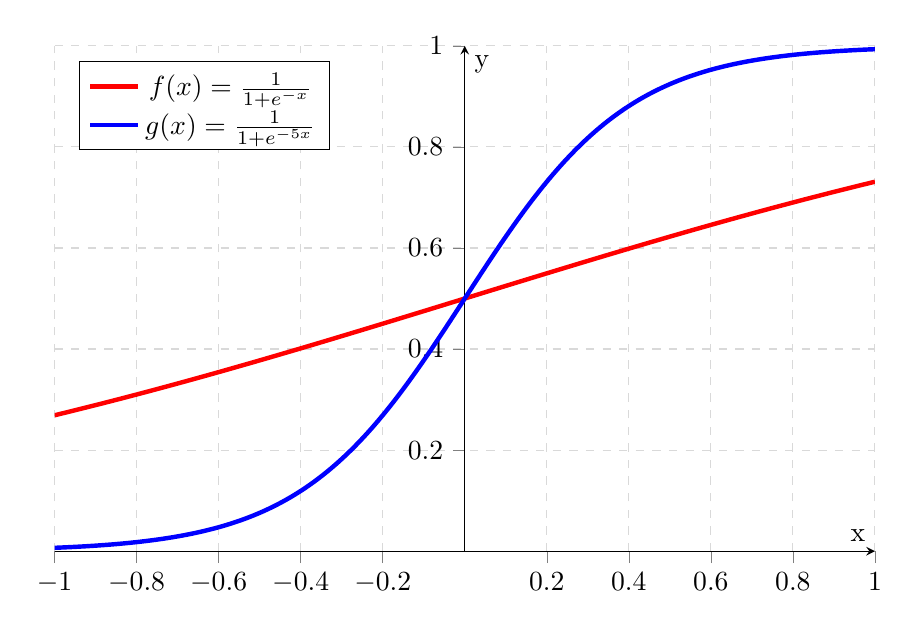
\begin{tikzpicture}
    \begin{axis}[
    	legend pos=north west,
        axis x line=middle,
        axis y line=middle,
        grid = major,
        width=12cm,
        height=8cm,
        grid style={dashed, gray!30},
        xmin=-1,     % start the diagram at this x-coordinate
        xmax= 1,    % end   the diagram at this x-coordinate
        ymin= 0,     % start the diagram at this y-coordinate
        ymax= 1,   % end   the diagram at this y-coordinate
        %axis background/.style={fill=white},
        xlabel=x,
        ylabel=y,
        tick align=outside,
        enlargelimits=false]
      % plot the stirling-formulae
      \addplot[domain=-1:1, red, ultra thick,samples=500] {1/(1+exp(-x))}; 
      \addplot[domain=-1:1, blue, ultra thick,samples=500] {1/(1+exp(-5*x))}; 
      \addlegendentry{$f(x)=\frac{1}{1+e^{-x}}$}
      \addlegendentry{$g(x)=\frac{1}{1+e^{-5x}}$}
    \end{axis} 
\end{tikzpicture}

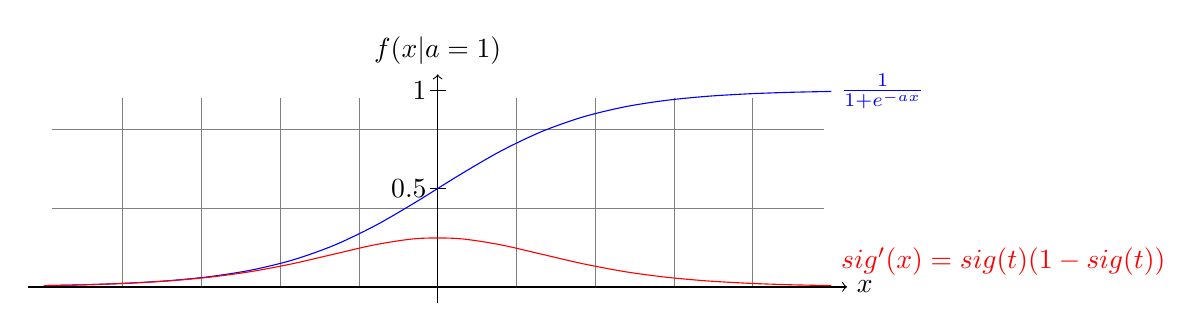
\begin{tikzpicture}[domain=-5:5, smooth, samples=20]
	\draw[very thin, color=gray] (-4.9,0.0) grid (4.9,2.4);

	\draw[->] (-5.2,0) -- (5.2,0) node[right] {$x$};
	\draw[->] (0,-0.2) -- (0,2.7) node[above] {$f(x|a=1)$};
	\draw (-0.1,2.5) --(0.1,2.5) node [left] {$1~$};
	\draw (-0.1,1.25) -- (0.1,1.25) node [left] {$0.5~$};

	\draw[color=blue] plot (\x,{2.5 / (1+exp(-\x))}) node[right] {$\frac{1}{1+e^{-ax}}$};
	\draw[color=red]  plot (\x,{2.5 / (1+exp(-\x)) * (1-1/(1+exp(-\x)))}) node[above right] {$sig'(x)=sig(t)(1-sig(t))$};
\end{tikzpicture}

\subsection{Derivation}

\begin{itemize}

\item Uses Delta learning rule

\begin{align*}
\Delta w = \eta r x \\
rx = \Delta E \\
\Delta w = - \eta \Delta E \\
\end{align*}

\item It follows gradient descent method

\def\layersep{3.5cm}
\begin{figure}[ht!]
\caption{An Multi Layer Backpropagation Network} 
\label{fig:an_multi_layer_backpropagation}
\centering
\begin{tikzpicture}[shorten >=1pt,->,draw=black!20, node distance=\layersep]
    % Draw the input layer neurons
    \node[input neuron] (I-1) at (0,-1) {$x_1$};
    \node[input neuron] (I-2) at (0,-2) {$x_i$};
    \node[input neuron] (I-3) at (0,-3) {$x_n$};
    
    % Draw the hidden layer neurons
    \node[hidden neuron] (H-1) at (2,-1) {$z_1$};
    \node[hidden neuron] (H-2) at (2,-2) {$z_j$};
    \node[hidden neuron] (H-3) at (2,-3) {$z_p$};
    
    \node[hidden neuron] (B-0) at (.5,-4) {$x_0$};

    \node[output neuron] (O-1) at (4, -1) {$y_1$};
    \node[output neuron] (O-2) at (4, -2) {$y_k$};
    \node[output neuron] (O-3) at (4, -3) {$y_m$};
    
    \node[hidden neuron] (B-1) at (2.5,-4) {$z_0$};

    % Connect every node in the input layer with the output layer
    \foreach \InputLayerNeuron in {1,...,3}
    	\foreach \HiddenLayerNeuron in {1,...,3}
        	\path (I-\InputLayerNeuron)  edge (H-\HiddenLayerNeuron);	

     \foreach \HiddenLayerNeuron in {1,...,3}
     \foreach \OutputLayerNeuron in {1,...,3}
        	\path (H-\HiddenLayerNeuron)  edge (O-\OutputLayerNeuron);
        	
     %\node[output neuron,pin={[pin edge={->}]right:Output}, right of=I-2] (Output) {o};
     \draw[thick, ->] (O-2) -- (6, -2) node[above] {$O_{jk}$} ;
     % Connect every node in the input layer with the output layer
    \foreach \HiddenLayerNeuron in {1,...,3}
    		\path (B-0)  edge (H-\HiddenLayerNeuron);
    
     \foreach \OutputLayerNeuron in {1,...,3}
        	\path (B-1)  edge (O-\OutputLayerNeuron);
        	
    % Annotate the layers and weigths
    \node[annot] at(-0.5, -5) {Input layer};
    \node[annot] at(2, -5) {Hidden layer};
    \node[annot] at(4.5, -5) {Output layer};
    
    \path (I-1) edge node[above] {$V_{11}$} (H-1);
    \path (I-2) edge node[above] {$V_{ij}$} (H-2);
    \path (I-3) edge node[above] {$V_{np}$} (H-3);
    
    \path (H-1) edge node[above] {$W_{11}$} (O-1);
    \path (H-2) edge node[above] {$W_{jk}$} (O-2);
    \path (H-3) edge node[above] {$W_{pm}$} (O-3);
\end{tikzpicture}
\end{figure}

\item If bias is not included in the network the activation fuction 
\[
f(net) = \begin{cases}
          \matplus1 & Net > \theta \\
          -1        & Net < \theta
          \end{cases}
\]
\[
Net = \sum w^Tx
\]
\item If bias is included we assume $\theta = 0$
\[
f(net) = \begin{cases}
          	\matplus1 & Net > 0 \\
          	-1 		  & Net < 0
          \end{cases}
\]
\end{itemize}

% Use & to align the equation to the left marigin
\section{Weight Updation in Output Layer}
\begin{align*}
& W_{jk}(t+1) = W_{jk}(t) + \Delta W_{jk}  \\ 
& \Delta W_{jk} = \eta r x  \\
& \text{In delta rule}  \\
& r = (d_i - O_i) f'(Net)  \\
& \Delta W_{jk}= \eta (t_k - O_{jk}) f' (O_{jk})O_{jk}  \\
\end{align*}
\begin{align}
\Delta W_{jk} = \eta (t_k - O_{jk}) O_{jk}(1-O_{jk})O_{ij}
\end{align}

\subsection{Proof:}

\begin{align*}
&E = t_k - O_{j,k} \\
&By Least Mean Square \\
&E = \frac{1}{2}(t_k-O_{jk})^2 \\
&O_{jk} = f(Net_{jk})
\end{align*}

\begin{align}
Net_{jk} = \sum W_{jk} \times O{jk}
\end{align}

According to delta learning rule

\begin{align*}
\Delta W &= - \eta \Delta E \\
\Delta W_{jk} &= - \eta \frac{\partial \Delta E}{\partial W_{j,k}} \\
\end{align*}

\begin{align}
\frac{\partial \Delta E}{\partial W_{j,k}} &= \frac{\partial \Delta E}{\partial Net_{j,k}} \times
                                             \frac{\partial Net_{j,k}}{\partial W_{j,k}} 
\end{align}  
\begin{align*}                                        
\Delta W_{jk} &= - \eta \frac{\partial \Delta E}{\partial Net_{j,k}} \times
                   \frac{\partial Net_{j,k}}{\partial W_{j,k}} \\
              &= - \frac{\partial \Delta E}{\partial Net_{j,k}} \times
                   \frac{\partial Net_{j,k}}{\partial W_{j,k}} \\
\text{By considering~~~~}  \eta = -1 \\
		      &=  \delta_{jk} \times
                  \frac{\partial Net_{jk}}{\partial W_{jk}} \\
\frac{\partial Net_{jk}}{\partial W_{jk}} &= \frac{ \partial \sum W_{jk} O_{ij}}{\partial W_{jk}} \\
										  &= O_{ij} \\
\Delta W_{jk} &= \delta_{jk} O_{ij} \\
\delta _{jk}       &= - \frac{\partial E}{\partial Net_{jk}} \\
\text{By chain rule}  \\
\delta_{jk}   &= - \frac{\partial E}{\partial O_{jk}} \times \frac{\partial O_{jk}}{\partial Net_{jk}} \\
\frac{\partial E}{\partial O_{jk}} &= \frac{\partial \frac{1}{2}(t_k - O_{jk})^2}{\partial O_{jk}} \\
			  &= -t_k + O_{jk} \\
\frac{\partial O_{jk}}{\partial Net_{jk}} &= \frac{\partial F(Net_{jk})}{\partial Net_{jk}} \\
										  &= F'(Net_{jk}) \\
										  &= O_{jk} (1-O_{jk}) \\
\delta_{jk} &= (t_k - O_{jk})O_{jk}(1-O{jk}) \\
\Delta      &= (t_k - O_{jk})O_{jk}(1-O_{jk})O_{ij}
\end{align*} 

\subsection{Weight  Updation in the Hidden Layer}
\begin{align*}
\Delta V_{ij} = \eta~\delta_{ij}~x \\
\delta_{ij} &= - \frac{\partial \Delta E}{\partial Net_{ij}} \\
       &= - \frac{\partial \Delta E}{\partial O_{ij}} \times \frac{O_{ij}}{\partial Net_{ij}} \\
       &= - \frac{\partial \Delta E}{\partial Net_{jk}} \times \frac{\partial Net_{jk}}{\partial O_{ij}} \times \frac{\partial}{\partial Net_{ij}} f(Net_{ij}) \\
       &= - \delta_{jk} \times \frac{\partial}{\partial O_{ij}} \sum W_{jk} O_{ij} \times f'(Net_{ij}) \\
       &= - \delta_{jk} \times \sum W_{jk} \times O_{ij}(1-O_{ij}) \\
\Delta V_{ij} = \eta~\delta_{jk} ~ \sum W_{jk} ~ O_{ij}(1-O_{ij})~x
\end{align*}
\section{Algorithm}
\begin{enumerate}
\item Initialize the weights
\item Choose proper activation function
\item For each training input vector do the following steps until $\Delta w = 0$
\begin{enumerate}
\item Calculate the net value of hidden layer using inputs and weights \\
$ Net_{i,j} = \sum V_{i,j}x_i $
\item Apply activation function and find output of hidden layer or input of output layer \\
$ O_{i,j} = f(Net_{i,j}) $
\item Calculate the Net value of the output layer \\
$ Net_{i,j} = \sum W_{i,j} O_{i,j} $
\item Apply activation function and find output of output layer \\
$ O_{j,k} = f(Net_{j,k}) $ 
\item Calculate the error $E = t_k - O_{j,k} $, using LMS error principle
\item Calculate the portion of the error $ \partial_{jk} $ which has to be back propagated to the hidden layer \\
$ \partial_{jk} = - \frac{\partial E}{\partial Net_{jk}} $ \\
$          ~~~~~= (t_k - O_{jk}) O_{jk}(1-O_{jk}) $
\item Adjust the weights $\Delta W_{jk} = \eta \partial_{jk} O_{ij} $
\item Calculate the portion of the error $ \partial_{ij} $ that has to be back propagated to input layers \\
$ \partial_{ij} = \partial_{jk} \sum (W_{jk})O_{ij}(1-O_{ij}) $
\item Adjust the weights 
\item Check for weight convergence
\end{enumerate}
\end{enumerate}


\chapter{Reference Links}

\section{Backpropagation:}
\url{http://en.wikipedia.org/wiki/Delta_rule} \\
\url{http://en.wikipedia.org/wiki/Backpropagation} \\ 
\url{https://www4.rgu.ac.uk/files/chapter3\%20-\%20bp.pdf} \\ 
\url{http://docs.opencv.org/modules/ml/doc/neural_networks.html} \\ 


\section{Maths}
\url{http://en.wikipedia.org/wiki/Partial_derivative} \\
\url{http://en.wikipedia.org/wiki/Gradient_descent} \\
\url{http://en.wikipedia.org/wiki/Chain_rule} \\
\url{http://en.wikipedia.org/wiki/Power_rule} \\

